\documentclass[11pt, aspectratio = 169]{beamer}

\usetheme[progressbar=frametitle]{metropolis}
\usepackage{appendixnumberbeamer}
\usepackage{booktabs}
\usepackage[scale=2]{ccicons}
\usepackage{pgfplots}
\usepgfplotslibrary{dateplot}
\usepackage{xspace}
\usepackage{comment}
\usepackage{cancel}
\usepackage{hyperref}  
\usepackage[dvipsnames]{xcolor}
    \definecolor{myteal}{HTML}{008080}
    \definecolor{myorange}{HTML}{E67E22}
    \definecolor{mypetrol}{HTML}{005F6A}
    \definecolor{mycyan}{HTML}{2AA8A1}
    \definecolor{mygold}{HTML}{D4A017}
    \definecolor{myrust}{HTML}{C65D32}
    \definecolor{mygrey}{HTML}{4D4D4D}
    \definecolor{mylightgrey}{HTML}{D9D9D9}
\usepackage{tikz}  
\usetikzlibrary{shapes,decorations,arrows,calc,arrows.meta,fit,positioning}
\tikzset{
    -Latex,auto,node distance =1 cm and 1 cm,semithick,
    state/.style ={ellipse, draw, minimum width = 0.7 cm},
    point/.style = {circle, draw, inner sep=0.04cm,fill,node contents={}},
    bidirected/.style={Latex-Latex,dashed},
    el/.style = {inner sep=2pt, align=left, sloped}
}
\usepackage{verbatim} 
\usepackage{listings}
\newcommand{\themename}{\textbf{\textsc{metropolis}}\xspace}
\definecolor{links}{HTML}{1B1B81}
\hypersetup{colorlinks,linkcolor=blue,urlcolor=blue}

% listings: To highlight code:
\usepackage{listings}
\lstset{
  language=R,
  basicstyle=\ttfamily\footnotesize,
  keywordstyle=\color{blue},
  commentstyle=\color{green!50!black},
  stringstyle=\color{red},
  frame=single,
  showstringspaces=false
}
\lstset{basicstyle=\ttfamily\footnotesize, frame=single}

\title{Applied Economics}
\subtitle{Instrumental Variables}
\author{Pello Aspuru}
\date{}
\institute{Winter 2025/26}
% \titlegraphic{\hfill\includegraphics[height=1.5cm]{logo.pdf}}
\setbeamercolor{normal text}{fg=black}
\setbeamercolor{block title}{fg=teal}
\setbeamercovered{transparent} % default faintness (~15%)

\let\svdescription\description
\let\svenddescription\enddescription
\renewenvironment{description}{%
  \svdescription%
  \let\svitem\item%
  \renewcommand\item[1][]{\svitem[\textcolor{\descriptioncolor}{##1}]}%
  }{
  \svenddescription%
  }
\newcommand\descriptioncolor{teal}

%\usepackage{Sweave}
\begin{document}
%\Sconcordance{concordance:AE_w8_IV.tex:AE_w8_IV.Rtex:%
1 45 1 1 0 525 1}


\maketitle
\sffamily

\begin{comment}
\begin{frame}{Plan for this Lecture}
\begin{enumerate}

%\item Homework Assignment 2

\item Simple Case: Bivariate Regression with one instrument

\item Example in R

\item General Case: Multivariate Regression with one or more endogenous regressors

\item Example in R

\end{enumerate}
\end{frame}
\end{comment}

%\section{Homework 2}

%\section{IVs}

\begin{frame}[fragile]{Motivation}

\begin{center}
    Does having children \alert{cause} a decrease in working hours?
\end{center}
\pause
Single Linear Regression Statistical model for the population:
\[
Y_{i} = \beta_0 + \alert{\beta_1} X_{1i} + u_i \quad i=1,...,N
\]
\begin{lstlisting}[language=R]
    library(wooldridge)
    data("labsup")
    mlr_labsup <- lm(hours ~ kids, data = labsup)
\end{lstlisting}
\pause

\begin{itemize}
    \item Exogeneity $E[u_i | X_{1i}] = 0$ \pause $\rightarrow$ \alert{$\hat{\beta}_1^{OLS}$} is consistent \& unbiased.
    \item Endogeneity $E[u_i | X_{1i}] \neq 0$ \pause $\rightarrow$ \alert{$\hat{\beta}_1^{OLS}$} is inconsistent \& biased.
\end{itemize}
\pause
Instrumental Variable (IV) estimation is an approach to get a consistent \& unbiased estimator \alert{$\hat{\beta}_1$} even if $X_{1i}$ is exogenous \pause $\rightarrow$ causal inference.
\end{frame}


\begin{frame}{Illustration: Instrumental Variables (IV) approach}

$X_{1i}$ is exogenous if it is not correlated with the error term $u_i$, \onslide<2->{ otherwise endogenous.}
\vspace{1mm}
\begin{block}{\onslide<3->{Instrumental Variable $Z_i$}}
    \onslide<3->{
    $Z_i$ is \textbf{correlated with the endogenous regressor $X_{1i}$}, \textbf{but uncorrelated with $u_i$}}
    \vspace{-1mm}
    \onslide<4->{
    \begin{itemize}
        \item \textcolor{mygold}{First Stage} $Z_i$ decomposes $X_{i}$'s variation into  endogenous $v_i$ and exogenous $\hat{X}_i$.
        \item \textcolor{mycyan}{Second Stage} Use $X_i$'s exogenous variation to obtain a consistent estimate $\hat{\beta}^{IV}$.
    \end{itemize}}
\end{block}
\vspace{2mm}
\begin{columns}
    \begin{column}{0.2\linewidth}
    \centering
    \onslide<1->{
        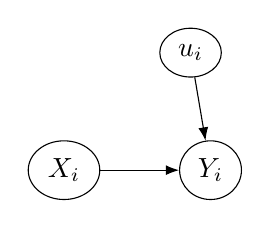
\begin{tikzpicture}
    % x node set with absolute coordinates
    \node[state] (x) at (0,0) {$X_i$};

    % y node set relative to x.
    % Locations can be:
    % right,left,above,below,
    % above left,below right, etc
    \node[state] (y) [right =of x] {$Y_i$};
    \node[state] (u) [above right =of x] {$u_i$};

    % Directed edge
    \path (x) edge (y);
    \path (u) edge (y);

    % Bidirected edge
   % \path[bidirected] (x) edge[bend left=60] (y);
    \end{tikzpicture}}
    \end{column}
    \begin{column}{0.2\linewidth}
\centering
\onslide<2->{
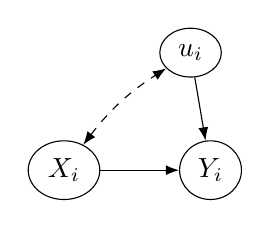
\begin{tikzpicture}
    % x node set with absolute coordinates
    \node[state] (x) at (0,0) {$X_i$};

    % y node set relative to x.
    % Locations can be:
    % right,left,above,below,
    % above left,below right, etc
    \node[state] (y) [right =of x] {$Y_i$};
    \node[state] (u) [above right =of x] {$u_i$};

    % Directed edge
    \path (x) edge (y);
    \path (u) edge (y);

    % Bidirected edge
    \path[bidirected] (x) edge[bend left=10] (u);    
\end{tikzpicture}}
    \end{column}
    \begin{column}{0.5\linewidth}
\centering
\onslide<3->{
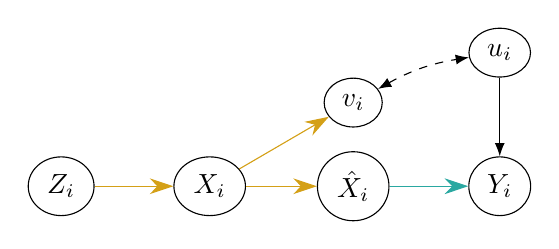
\begin{tikzpicture}

    % Nodes
    \node[state] (x) at (-1,0) {$X_i$};
    \node[state] (xh) [right=0.9cm of x] {$\hat{X}_i$};
    \node[state] (v) [above=0.3cm of xh] {$v_i$};
    \node[state] (z) [left =of x] {$Z_i$};
    \node[state] (y) [right =of xh] {$Y_i$};
    \node[state] (u) [above =of y] {$u_i$};

    % Colored edges (full arrow color)

    % X → Xhat (changed to mygold)
    % X → v (changed to mygold)
    \path[-{Stealth[length=3mm,width=2mm]}, draw=mygold, fill=mygold]
        (x) edge (xh)
        (x) edge (v);

    % Xhat → Y (still mycyan)
    \path[-{Stealth[length=3mm,width=2mm]}, draw=mycyan, fill=mycyan]
        (xh) edge (y);

    % u → y
    \path (u) edge (y);

    % Z → X (still mygold)
    \path[-{Stealth[length=3mm,width=2mm]}, draw=mygold, fill=mygold]
        (z) edge (x);

    % Bidirected dashed arrow Z ↔ u in mypetrol
    %\path[bidirected, dashed, draw=mypetrol, fill=mypetrol]
        %(z) edge[bend left=15] (u);

    % Bidirected edge v ↔ u
    \path[bidirected] (v) edge[bend left=10] (u);

\end{tikzpicture}}
    \end{column}
\end{columns}
\vspace{2mm}
\onslide<5->{
\begin{itemize}
    \item[$\rightarrow$] What correlates with \# of kids, but does not correlate with working hours? 
\end{itemize}

}

\end{frame}



\begin{frame}{Regression with one Endogenous Regressor and one Instrument}
Instrument $Z_i$ is an indicator variable that turns on if the first two kids are same sex.
\pause
\begin{align*}
    Y_{i} &= \beta_0 + \beta_1 X_{1i} + u_i \quad &\text{ with } E[X_{1i}u_i] \neq 0 
    \\
    X_{1i} &= \pi_0 + \pi_1 Z_i + v_{i } \quad &\text{ with } E[Z_iu_i] = 0 
\end{align*}
\pause
A variable $Z_i$ is a \textbf{suitable instrument} for $X_{1i}$ if it satisfies two conditions:
\pause
\begin{columns}[T]

% ---------------- Left column ----------------
\begin{column}{0.7\textwidth}

\begin{enumerate}
    \item \textcolor{mygold}{\textbf{Relevance}}: $ \operatorname{cov}(Z_i, X_{1i}) \neq 0 $ \\
          Instrument $Z_i$ ``drives'' endogenous covariate $X_{1i}$. \\
          $\rightarrow$ can be used to extract \textcolor{teal}{variation} in $X_i$.
    \item \textcolor{mypetrol}{\textbf{Exogeneity}}: $ \operatorname{cov}(Z_i, u_i) = 0 $ \\
          Instrument is (as if) randomly allocated. \\
          $\rightarrow$ The \textcolor{teal}{variation} we extract is \textbf{exogenous}.
\end{enumerate}

\end{column}

% ---------------- Right column ----------------
\begin{column}{0.3\textwidth}

\begin{center}
\vspace*{\fill}

\resizebox{0.95\linewidth}{!}{%
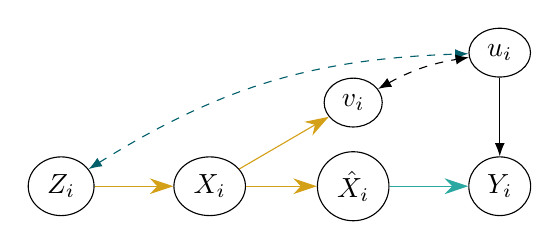
\begin{tikzpicture}

    % Nodes
    \node[state] (x) at (-1,0) {$X_i$};
    \node[state] (xh) [right=0.9cm of x] {$\hat{X}_i$};
    \node[state] (v) [above=0.3cm of xh] {$v_i$};
    \node[state] (z) [left =of x] {$Z_i$};
    \node[state] (y) [right =of xh] {$Y_i$};
    \node[state] (u) [above =of y] {$u_i$};

    % Colored edges (full arrow color)

    % X → Xhat (changed to mygold)
    % X → v (changed to mygold)
    \path[-{Stealth[length=3mm,width=2mm]}, draw=mygold, fill=mygold]
        (x) edge (xh)
        (x) edge (v);

    % Xhat → Y (still mycyan)
    \path[-{Stealth[length=3mm,width=2mm]}, draw=mycyan, fill=mycyan]
        (xh) edge (y);

    % u → y
    \path (u) edge (y);

    % Z → X (still mygold)
    \path[-{Stealth[length=3mm,width=2mm]}, draw=mygold, fill=mygold]
        (z) edge (x);

    % Bidirected dashed arrow Z ↔ u in mypetrol
    \path[bidirected, dashed, draw=mypetrol, fill=mypetrol]
        (z) edge[bend left=15] (u);

    % Bidirected edge v ↔ u
    \path[bidirected] (v) edge[bend left=10] (u);

\end{tikzpicture}
}%

\vspace*{\fill}
\end{center}

\end{column}

\end{columns}
\vspace{2mm}
\pause
\begin{center}
    What does \textit{extract variation} mean?
\end{center}
\end{frame}

\begin{frame}[fragile]{Two-Stage Least Squares (2SLS)}
The Two Stage Least Square estimator \textbf{illustrates} the intuition of the IV Approach.
\\
\vspace{2mm}
\pause
\color{teal}\textbf{First Stage}: \color{black} 
\begin{itemize}
    \item Test instrument $Z_i$'s \textbf{relevance}: $X_{1i} = \pi_0 + \pi_1 Z_i + v_i$.
    \begin{lstlisting}[language=R]
    first_stage <- lm(kids ~ samesex, labsup)
    \end{lstlisting}
    \pause
    \item Compute fitted values $\alert{\hat{X}_{1i} }= \pi_0 + \pi_1 Z_i$.
    \begin{lstlisting}[language=R]
    labsup$fitted_kids <- first_stage$fitted.values
    \end{lstlisting}
\end{itemize}
\pause
%\vspace{+0.15cm}
\color{teal} \textbf{Second Stage}: \color{black} 
\begin{itemize}
    \item Estimate regression $Y_{i} = \beta_0 + \beta_1 \alert{\hat{X}_{1i}} + u_i$
    \begin{lstlisting}[language=R]
    second_stage <- lm(hours ~ fitted_kids, data = labsup)
    \end{lstlisting}
    \item[$\rightarrow$] OLS estimation of the second stage model yields 2SLS estimator $\hat{\beta}^{2SLS}_0, \: \hat{\beta}^{2SLS}_1$
\end{itemize}

\end{frame}


\begin{frame}{2SLS estimator: Properties}
Under the assumptions of 
\begin{itemize}
    \item Linearity in parameters (Assumption 1)
    \item An i.i.d.\ random sample (Assumption 2)
    \pause
    \item Instrument relevance (instead of Assumption 3)
    \begin{itemize}
        \item[$\rightarrow$] Testable condition: First Stage.
    \end{itemize}
    \item Instrument exogeneity (instead of Assumption 4)
    \begin{itemize}
        \item[$\rightarrow$] Non-testable condition, needs to be argued. 
    \end{itemize}
\end{itemize}
\begin{center}
The 2SLS estimator yields \textcolor{teal}{consistent and asymptotically normal} point estimates.    
\end{center}
\end{frame}

\begin{frame}[fragile]{IV Identification and Estimation - Derivation}
The effect of the instrument $Z_i$ on outcome $Y_i$ is only through regressor $X_i$:
\begin{align*}
\operatorname{Cov}(Z_i, Y_i)
    &= \operatorname{Cov}(Z_i, \beta_0 + \beta_1 X_i + u_i) = \beta_1 \operatorname{Cov}(Z_i, X_i)
       + \cancelto{0}{\operatorname{Cov}(Z_i, u_i)} 
\end{align*}
\[\beta_1 = \frac{\operatorname{Cov}(Z_i, Y_i)}{\operatorname{Cov}(Z_i, X_i)}\]
\pause 
\vspace{-6mm}
\begin{itemize}
    \item This identifies the population parameter $\beta_1$.
    \item Using the sample analogue yields the \alert{IV Estimator}: $\hat{\beta}_1^{IV} = \frac{\widehat{Cov}(Z_i, Y_i)}{\widehat{Cov}(Z_i, X_i)}$
\end{itemize}
\vspace{3mm}
\pause
\begin{lstlisting}[language=R]
    library(estimatr)
    slr_iv <- iv_robust(hours ~ kids | samesex, 
                    data = labsup, se_type = "HC0", diagnostics = TRUE)
\end{lstlisting}
\end{frame}

\begin{frame}[fragile]{Variance of the IV Estimator - Intuition}
Why do variances of $\hat\beta_1^{2SLS}$ and $\hat\beta_1^{IV}$ differ?
\begin{lstlisting}[language=R]
    coeftest(second_stage, vcov. = vcovHC(second_stage, "HC0")) 
    summary(slr_iv)
\end{lstlisting}
\pause
Variances of $\hat\beta_1^{2SLS}$ and $\hat\beta_1^{IV}$ 
under conditional \emph{homoskedasticity} $E[u_i^2 \mid Z_i] = \sigma_u^2$:
\vspace{-1.5mm}
\[
\operatorname{Var}(\hat\beta_1^{2SLS}) 
    = \frac{\sigma_u^2}{n \cdot \sigma_{\hat X}^2}
\qquad
\operatorname{Var}(\hat\beta_1^{IV}) 
    = \frac{\sigma_u^2}{n \cdot \sigma_X^2 \cdot \textcolor{teal}{\rho_{x,z}^2}}
\]
Both in error variance $\sigma_u^2$,
decrease in sample size $n$, and in the variance of the regressor $\sigma_X^2$. 
\pause $\hat\beta_1^{IV}$ features additional term \color{teal}{$\rho_{x,z}$}\color{black}: the population \textbf{correlation} between $X$ and $Z$.

Since $\rho_{x,z} < 1$, the IV variance is \textbf{\alert{larger}}
$\operatorname{Var}(\hat\beta_1^{OLS})$.

\begin{itemize}
    \item because we only use a \textbf{part} of the total variation in $X_i$ in the IV estimation.
    \item the stronger the correlation between $X$ and $Z$, the smaller is the increase.
    \item[$\rightarrow$] 2SLS procedure underestimates parameter estimate variances!
\end{itemize}

\end{frame}

\begin{frame}{Instrument Relevance and Weak Instruments}
    If the correlation betw. $Z_i$ and $X_i$ is small, we have a \alert{weak instrument} problem, that yields very imprecise IV estimates


    Rule of thumb for sufficiently strong instrument:  F-statistic in the first stage $>$ 10.

    New research suggests that the threshold value for the
F-test should be chosen much larger in practice, $\approx$ 104.
    \bigskip


\pause 
Weak instruments are also an issue for consistency if exogeneity is not fully satisfied:
\begin{align*}
    plim(\hat{\beta}_1^{OLS}) &= \beta_1 + Cov (X, u)/Var(X)   \\
plim(\hat{\beta}_1^{IV}) &= \beta_1 + Cov (Z, u)/Cov(Z,X)
\end{align*}

IV estimator is consistent if exogeneity is satisfied: $Cov(Z, u) = 0$

If exogeneity does not hold, inconsistency of IV is stronger the weaker the correlation of $Z$ and $X$!

%If inconsistency in OLS is not strong (cov(x, u) small) it can be better to use OLS than a weak instrument. 

\end{frame}

\begin{frame}{Tradeoffs between OLS and IV}

If Assumption 4 is violated, we can choose between inconsistent, but precise OLS estimator and a consistent, but less precise IV estimator. \\
$\rightarrow$ \textbf{\alert{Bias–Variance-Tradeoff}}
\pause
Best choice depends on context.
\begin{itemize}
    \item Do IV if you think endogeneity is sufficiently important. \\
    Otherwise, inconsistency of OLS is small, and it might still be close to the true value; whereas IV is correct in infinite samples, but might be pretty far off the true value in finite samples.
    \item Try to find \textbf{strong} instruments, e.g. in the bivariate case an IV where  $|corr(X_i, Z_i)|$ is large. \pause
    \item[$\rightarrow$] In practice, report \textbf{both} OLS and IV estimates. 
\end{itemize}
\end{frame}

\begin{comment}
    \section{Example in R - Causal Effect of Education on Wages}
\end{comment}

\begin{comment}
    \begin{frame}[fragile]{Education and wage again}

\begin{lstlisting}[language=R]
    library(wooldridge)
    library(sandwich)
    library(lmtest)
    library(car)
    data("mroz")  # data on education and wages of married women in the US
\end{lstlisting}

\begin{lstlisting}[language=R]
    mroz <- mroz[!is.na(mroz$lwage), ]
\end{lstlisting}

Estimate simple regression model by \textbf{OLS}
\small
\begin{lstlisting}[language=R]
    ols_est <- lm(lwage ~ educ, data = mroz)
    coeftest(ols_est, vcov. = vcovHC(ols_est, "HC1"))  
\end{lstlisting}

One additional year of education on average associated with increase in wage by 10.9\%

\end{frame}
\end{comment}

\begin{comment}
    \begin{frame}[fragile]{Using maternal education as an IV}
    Is mother's education a suitable instrument?

    \pause

    \textbf{First Stage} Regression \textcolor{teal}{(Relevance)}
    \small
    \begin{lstlisting}[language=R]
        first_st <- lm(educ ~ motheduc, data = mroz)
    coeftest(first_st, vcov. = vcovHC(first_st, "HC1"))  
    \end{lstlisting}
    \end{frame}
\end{comment}

\begin{comment}
    \begin{frame}[fragile]{Using maternal education as an IV}

    What about  \textcolor{teal}{exogeneity}?

    \end{frame}
\end{comment}

\begin{comment}

\begin{frame}[fragile]{Using maternal education as an IV}
\textbf{Second Stage} Regression \textit{(manually)}
\small
\begin{lstlisting}[language=R]
    mroz$fitted_educ <- first_st$fitted.values # get fitted values from first stage
    second_st <- lm(lwage ~ fitted_educ, data = mroz)
    coeftest(second_st, vcov. = vcovHC(second_st, "HC1"))  
\end{lstlisting}
\vspace{-0.29cm}
One additional year of education on average increases wage by 3.9\% $\rightarrow$  less than OLS estimate (which is likely biased upward). 

\normalsize
\alert{When running the two stages separately,  standard errors in the 2. stage are incorrect!}
\end{frame}

\begin{frame}[fragile]{Using maternal education as an IV}
\textbf{Using built-in IV estimator} gives correct standard errors
\small

\begin{lstlisting}[language=R]
    install.packages("estimatr") \\
    library(estimatr) \\
    tsls <- iv\_robust(lwage $\sim$ educ | motheduc, data = mroz, 
    se\_type = "HC1", diagnostics = T)
    summary(tsls)
\end{lstlisting}

\begin{tabular}{l|rrrrrrr}
\hline
term & estimate & std.error & statistic & p.value & conf.low & conf.high & df \\
\hline
(Intercept) & 0.702 & 0.494 & 1.422 & 0.156 & -0.268 & 1.673 & 426 \\
educ & 0.039 & 0.039 & 0.982 & 0.327 & -0.039 & 0.116 & 426 \\
\hline
\end{tabular}

\end{frame}

\begin{frame}{Practice}
    Run the First Stage Regression and get the IV estimate with  \texttt{\textcolor{teal}{iv\_robust()}} with $fatheduc$ as instrument.
    
    How do the results compare to the case with $motheduc$ as IV?
\end{frame}

\end{comment}

\section{General Case: Multiple regression model with one or more endogenous regressors}

\begin{frame}{General Case}

General linear model with endogeneity:
$Y_i = \boldsymbol{X}_i'\boldsymbol{\beta} + u_i,\; \text{ with } E[\boldsymbol{X}_i u_i] \neq \boldsymbol{0}$

We partition the elements of $\boldsymbol{X}_i$ {\color{gray}$(k \times 1)$} into
\begin{itemize}
    \item endogenous regressors $\boldsymbol{X}_{1i}$ {\color{gray}$(k_1 \times 1\text{ vector})$} which we try to instrument, and
    \item exogenous regressors $\boldsymbol{X}_{2i}$ {\color{gray}$(k_2 \times 1\text{ vector})$}
\end{itemize}

\vspace{0.15cm}
The exogenous regressors serve as ``instruments for themselves'': \\
\hspace{0.25cm}\alert{included instruments} $\boldsymbol{Z}_{2i} = \boldsymbol{X}_{2i}$ {\color{gray}$(k_2 \times 1)$} \\[0.1cm]
For the endogenous regressors, we need variables from outside the model as IVs: \\
\hspace{0.25cm}\alert{excluded instruments} $\boldsymbol{Z}_{1i}$ {\color{gray}$(l_1 \times 1)$}

\vspace{0.15cm}
We write the {\color{gray}$(l \times 1)$}-vector of instrumental variables:
\[
\boldsymbol{Z}_i = 
\begin{pmatrix}
    \boldsymbol{Z}_{1i} \\
    \boldsymbol{Z}_{2i}
\end{pmatrix}
\]

\end{frame}

\begin{frame}{Multiple Regression Model}
We \alert{need at least as many excluded instruments as endogenous regressors: $l_1 \geq k_1$} \\
If {$l_1 = k_1$} (as many IVs as endogenous regressors), the model is called \textit{just-identified}. \\
If {$l_1  > k_1$} (more IVs than endogenous regressors), the model is called \textit{over-identified}.

\bigskip

\begin{block}{Conditions for suitable IVs}
\begin{enumerate}
    \item Exogeneity: uncorrelated with error  $u_i$
    \item Relevance: \alert{partially} correlated with endogenous explanatory variable
\end{enumerate}
\end{block}
\end{frame}

\begin{frame}[fragile]{First Stage and Relevance}

\textbf{First stage regression(s)}:  For each \alert{endogenous} regressor $X_{ji}$, run a first stage regression of that regressor on all included \alert{\emph{and excluded}} instruments:
\begin{align*}
X_{ji} 
    = \pi_0 
    + \underbrace{\pi_1 Z_{1i} + \cdots + \pi_{l_1} Z_{l_1 i}}_{\text{excluded IVs}} 
    + \underbrace{\boldsymbol{X}'_{2i}\boldsymbol{\gamma}}_{\text{included IVs}} 
    + v_i,
    \qquad j = 1, \ldots, k_1.
\end{align*}
\pause
Estimate the first stage(s)... 
\begin{lstlisting}[language=R]
    mlr_first_stage <- lm( kids ~ samesex + age + educ, labsup)
\end{lstlisting}
\pause
... and obtain the fitted values of the endogenous regressor(s): $(\hat{X}_{1i}, ..., \hat{X}_{ki})'$.
\begin{lstlisting}[language=R]
    labsup$fitted_kids <- mlr_first_stage$fitted.values
\end{lstlisting}

\end{frame}

\begin{frame}[fragile]{Second Stage}
In the second stage, we regress the dependent variable $Y_i$ on the predicted values of all endogenous regressors, all exogenous variables and an intercept using OLS. 
\begin{align*}
Y_{i} = \beta_0 + \beta_1\hat{X}_{1i} + ... + \beta_{k} \hat{X}_{k i} + \boldsymbol{X}'_{2i}\boldsymbol{\beta}_{2} + u_i
\end{align*}
\pause
\begin{lstlisting}[language=R]
    mlr_second_stage <- lm(hours ~ fitted_kids + age + educ, labsup)
    coeftest(mlr_second_stage, vcov. = vcovHC(mlr_second_stage, "HC0"))  
\end{lstlisting}
This gives ($\hat{\beta}^{2SLS}_{0}$,$\hat{\beta}^{2SLS}_{1}$, ... $\hat{\beta}^{2SLS}_{k}$)', the 2SLS estimates of the model coefficients. \\
\pause
\vspace{3mm}
$\rightarrow$ Remember: the previous procedure yields:
\begin{itemize}
    \item Consistent parameter estimates.
    \item Incorrect parameter variance estimates.
\end{itemize}
\end{frame}

\begin{frame}[fragile]{IV Estimator}
$\rightarrow$ Important! use the R package for robust IV for \alert{correct} variance estimates:
\vspace{2mm}
\begin{lstlisting}[language=R]
mlr_iv <- iv_robust(hours ~ kids + age + educ | samesex + age + educ, 
                    data = labsup, se_type = "HC0", diagnostics = TRUE)
summary(mlr_iv)
\end{lstlisting}

\end{frame}

\begin{comment}

\section{Example in R - Labor Supply}

\begin{frame}[fragile]{Multiple Regression with endogenous regressor in R}  
We are interested in the causal effect of the number of kids on maternal labor supply (in hours per week). 
\footnotesize

\begin{lstlisting}[language=R]
    data("labsup")   # load dataset on mothers, incl. number of kids and hours worked
    table(labsup$kids) # sample includes women with two or more kids 
    ols_labsup <- lm(hours ~ kids + age + agesq + educ + 
        black + hispan, data = labsup) # baseline model
\end{lstlisting}

\end{frame}

\begin{frame}[fragile]{Multiple Regression with endogenous regressor in R}  

\footnotesize
\begin{lstlisting}[language=R]
    coeftest(ols_labsup, vcov. = vcovHC(ols_labsup, "HC1"))
\end{lstlisting}
\normalsize
\vspace{-0.3cm}
Why could the OLS estimator of the coefficient on $kids$ be biased?
\end{frame}

\begin{frame}[fragile]{Multiple Regression with endogenous regressor in R}  
We want to use $samesex$ as IV, an indicator that takes value 1 if the first two kids of the women have the same sex. Do you think this is a suitable IV?
\pause
\scriptsize

\end{frame}

\begin{frame}{2SLS estimation in MLR}  
\small

\texttt{%
> library(estimatr) \\
> \textcolor{olive}{\# important: include all IVs + exogenous regressors behind the | !} \\
> tsls\_labsub <- iv\_robust(hours $\sim$ kids + age + agesq + educ + black + \\
\hspace{3.6em} hispan \;|\; samesex + age + agesq + educ + black + hispan, \\
\hspace{3.6em} data = labsup, se\_type = "HC1", diagnostics = TRUE) \\
> summary(tsls\_labsub)
}

\vspace{0.3cm}

\texttt{Coefficients:}

\begin{tabular}{lrrrrrrr}
\hline
term & estimate & std.error & statistic & p.value & conf.low & conf.high & df \\
\hline
kids & -5.120 & 3.056 & -1.675 & 0.094 & -11.110 & 0.870 & 31850 \\
age & 2.129 & 0.483 & 4.410 & 0.000 & 1.183 & 3.075 & 31850 \\
\multicolumn{8}{c}{\dots} \\
\hline
\end{tabular}

\vspace{0.3cm}

\texttt{Diagnostics:}

\begin{tabular}{lrrrr}
\hline
 & numdf & dendf & value & p.value \\
\hline
Weak instruments & 1 & 31850 & 45.763 & 1.36e-11*** \\
\hline
\end{tabular}

\end{frame}

\end{comment}

\end{document}
